\documentclass[11pt, oneside]{article}
\usepackage[margin=1in,letterpaper]{geometry}
\usepackage{times}
\usepackage{graphicx}
\usepackage{amssymb,amsmath}
\usepackage{array}
\usepackage{longtable}
\usepackage{color}
\usepackage[T1]{fontenc}
\usepackage{sectsty}
\usepackage{tikz}
\usepackage{pgfplots}
\pgfplotsset{compat=1.17}
\sectionfont{\fontsize{12}{12}\selectfont}
\subsectionfont{\fontsize{11}{11}\selectfont}
\subsubsectionfont{\normalsize\itshape\mdseries}

\renewcommand\labelitemi{{\boldmath$\cdot$}}

%%%%%%%%%%%%%%%%%%%%%%%%%%%%%%%%%%%%%
% Notation: vectors are bold (handwritten: underlined); unit vectors are \hat{\mathbf{x}}, etc.
% Following the master table (D2, D12), phasors carry a tilde: E(x,y,z,t) = Re[E~(x,y,z) e^{jwt}].
% Per the master table: phase velocity u_p (D15), +z amplitude E_x^+ (D16), Poynting vector in script S (D10);
% the handwriting uses v_p, E_x0, and a plain S.
%%%%%%%%%%%%%%%%%%%%%%%%%%%%%%%%%%%%%

\title{Ge 158 Lecture 2: Maxwell's Equations and EM Wave Propagation}
\author{Brent Minchew}
\date{}

\begin{document}
\maketitle

\noindent\textbf{Topics covered}
\begin{itemize}
	\item Maxwell's equations
	\item EM wave propagation in free space
	\item EM wave propagation in lossy materials
	\item Poynting vector in general media
\end{itemize}

%%%%%%%%%%%%%%%%%%%%%%%%%%%%%%%%%%%%%
\section{Review of constitutive parameters}

Recall from last lecture that we can describe the EM properties of a material using four parameters, only two of which are relevant for RS:
\begin{enumerate}
	\item $\bigstar$ $\varepsilon'\varepsilon_0$ is the electrical \emph{permittivity} $\rightarrow$ ability to store electric charge;
	\item $\bigstar$ $\sigma$ is the electrical \emph{conductivity} $\rightarrow$ ability to allow electric current;
	% NOTE: handwritten reads "mu = mu_0 = eps_0/c^2"; corrected to 1/(eps_0 c^2) because c = 1/sqrt(mu_0 eps_0)
	% (Lecture 1; Ulaby & Long 2014, Eq. 2.31). eps_0/c^2 ~ 9.9e-29, not 4 pi x 10^-7.
	\item $\mu$ is the magnetic \emph{permeability}; $\mu = \mu_0 = 1/(\varepsilon_0 c^2) = 4\pi\times10^{-7}$ H/m for virtually all RS applications;
	% NOTE: handwritten uses rho_v for charge density; written q_v so that rho is reserved for reflection
	% coefficients (Lecture 4 onward, following Ulaby & Long). Instructor decision, 2026-09-29.
	\item $q_v$ is the \emph{charge density}; $q_v = 0$ in RS applications.
\end{enumerate}
We group the two important terms into the complex-valued relative dielectric constant
\begin{equation}
	\label{e:dielectric}
	\varepsilon = \varepsilon' - j\varepsilon'', \qquad \text{where} \qquad \varepsilon'' = \frac{\sigma}{\omega\varepsilon_0}.
\end{equation}
% NOTE: added scope (instructor decision, 2026-09-29), consistent with Lecture 1.
Here $\sigma/(\omega\varepsilon_0)$ is the conduction contribution to $\varepsilon''$; polarization (relaxation) losses also contribute (Lecture 1). In this lecture, any $\varepsilon'' > 0$ (from conduction or otherwise) is what matters.

%%%%%%%%%%%%%%%%%%%%%%%%%%%%%%%%%%%%%
\section{Maxwell's equations}

I assume that everyone has some familiarity with classical electrodynamics and the four fundamental equations often called Maxwell's equations. If these are totally new to you, consider consulting any number of excellent texts on the topic: Griffiths, \emph{Introduction to Electrodynamics}; Purcell and Morin, \emph{Electricity and Magnetism}; etc.

\subsection{Gauss's law for electricity}

Gauss's law for electricity is
\begin{equation}
	\label{e:gauss_e}
	\nabla\cdot\mathbf{E} = \frac{q_v}{\varepsilon'\varepsilon_0},
\end{equation}
where $\mathbf{E}$ is the electric field intensity vector (units: V/m),
\begin{equation}
	\nabla = \left[\frac{\partial}{\partial x}, \frac{\partial}{\partial y}, \frac{\partial}{\partial z}\right] = \hat{\mathbf{x}}\frac{\partial}{\partial x} + \hat{\mathbf{y}}\frac{\partial}{\partial y} + \hat{\mathbf{z}}\frac{\partial}{\partial z},
\end{equation}
and $\nabla\cdot\mathbf{E}$ is the divergence of $\mathbf{E}$.

\subsubsection{Review of divergence}

The divergence is a description of how much a vector field spreads out (diverges) at a point (Figure~\ref{f:divergence}a--c).

\begin{figure}[h]
	\centering
	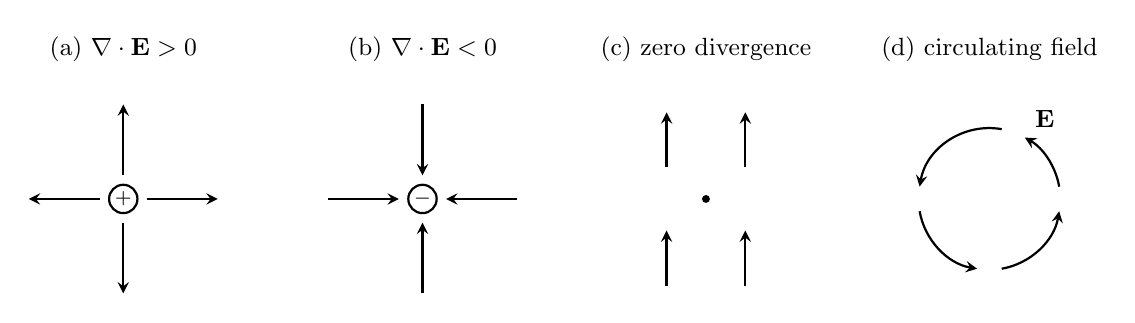
\begin{tikzpicture}[>=stealth, thick, font=\small]
		% (a) positive divergence
		\begin{scope}
			\node at (0,1.9) {(a) $\nabla\cdot\mathbf{E} > 0$};
			\draw (0,0) circle (0.18) node {\scriptsize $+$};
			\foreach \a in {0,90,180,270} \draw[->] (\a:0.3) -- (\a:1.2);
		\end{scope}
		% (b) negative divergence
		\begin{scope}[xshift=3.8cm]
			\node at (0,1.9) {(b) $\nabla\cdot\mathbf{E} < 0$};
			\draw (0,0) circle (0.18) node {\scriptsize $-$};
			\foreach \a in {0,90,180,270} \draw[->] (\a:1.2) -- (\a:0.3);
		\end{scope}
		% (c) zero divergence (uniform field)
		\begin{scope}[xshift=7.4cm]
			\node at (0,1.9) {(c) zero divergence};
			\fill (0,0) circle (0.05);
			\foreach \x in {-0.5,0.5} {
				\draw[->] (\x,0.4) -- (\x,1.1);
				\draw[->] (\x,-1.1) -- (\x,-0.4);
			}
		\end{scope}
		% (d) divergence-free circulating field
		\begin{scope}[xshift=11.0cm]
			\node at (0,1.9) {(d) circulating field};
			\draw[->] (80:0.9) arc (80:170:0.9);
			\draw[->] (190:0.9) arc (190:260:0.9);
			\draw[->] (280:0.9) arc (280:350:0.9);
			\draw[->] (10:0.9) arc (10:60:0.9) node[above right] {$\mathbf{E}$};
		\end{scope}
	\end{tikzpicture}
	\caption{(a) Positive divergence, (b) negative divergence, and (c) zero divergence of a vector field at a point. (d) An example of a divergence-free field that forms closed loops.}
	\label{f:divergence}
\end{figure}

\begin{itemize}
	\item So, in essence, Gauss's law says that a charge causes a flux through some closed surface.
	% NOTE: "like charges repel" is Coulomb's law rather than a direct statement of Gauss's law; kept as written.
	\item In other words, like charges repel, and the presence of a charge results in a diverging electric field.
	\item As noted before, $q_v = 0$ in RS applications $\Rightarrow$ electric fields are divergence-free!
	\item An example of a divergence-free field is shown in Figure~\ref{f:divergence}d.
\end{itemize}

\subsection{Gauss's law for magnetism}

\begin{equation}
	\label{e:gauss_m}
	\nabla\cdot\mathbf{H} = 0,
\end{equation}
where $\mathbf{H}$ is the magnetic field intensity vector (units: A/m).
\begin{itemize}
	\item Fun fact: there is no known magnetic ``charge'' $\Rightarrow$ magnetic fields are always divergence-free and tend to form closed loops.
\end{itemize}

\subsection{Faraday's law}

\begin{equation}
	\label{e:faraday}
	\nabla\times\mathbf{E} = -\mu\frac{\partial\mathbf{H}}{\partial t},
\end{equation}
where $\nabla\times\mathbf{E}$ is the curl of $\mathbf{E}$.

\subsubsection{Review of curl}

\begin{equation}
	\nabla\times\mathbf{E} =
	\begin{vmatrix}
		\hat{\mathbf{x}} & \hat{\mathbf{y}} & \hat{\mathbf{z}} \\[2pt]
		\dfrac{\partial}{\partial x} & \dfrac{\partial}{\partial y} & \dfrac{\partial}{\partial z} \\[8pt]
		E_x & E_y & E_z
	\end{vmatrix}
	= \left(\frac{\partial E_z}{\partial y} - \frac{\partial E_y}{\partial z}\right)\hat{\mathbf{x}}
	+ \left(\frac{\partial E_x}{\partial z} - \frac{\partial E_z}{\partial x}\right)\hat{\mathbf{y}}
	+ \left(\frac{\partial E_y}{\partial x} - \frac{\partial E_x}{\partial y}\right)\hat{\mathbf{z}}.
\end{equation}
The curl is a measure of the rotation of a vector field about a point.

\begin{itemize}
	% NOTE: handwritten reads "Time-varying magnetic field induces an electric field, and vice-versa"; the reverse (a time-varying E
	% inducing H) comes from Ampere's law with Maxwell's correction (next subsection), so "vice versa" is moved there.
	\item Faraday's law tells us that a time-varying magnetic field induces an electric field. (The reverse, a time-varying electric field inducing a magnetic field, comes from Amp\`ere's law with Maxwell's correction; see below.)
	% NOTE: handwritten reads "the E field forms closed loops (zero divergence, non-zero curl)". Zero divergence does not imply
	% closed loops (e.g., the straight field lines of a uniform plane wave, Section 3), and the curl of E is non-zero only where
	% dH/dt is non-zero.
	\item Together with Gauss's law for electricity, it tells us that in RS applications ($q_v = 0$) $\mathbf{E}$-field lines cannot begin or end on charges, and that a time-varying $\mathbf{H}$ gives $\mathbf{E}$ a non-zero curl (e.g., the closed loops of Figure~\ref{f:divergence}d).
\end{itemize}

\subsection{Amp\`ere's law (with Maxwell's correction)}

\begin{equation}
	\label{e:ampere}
	\nabla\times\mathbf{H} = \varepsilon'\varepsilon_0\frac{\partial\mathbf{E}}{\partial t} + \sigma\mathbf{E}.
\end{equation}
The first term on the right-hand side, $\varepsilon'\varepsilon_0\,\partial\mathbf{E}/\partial t$, was Maxwell's correction, and it leads directly to one of the greatest discoveries\ldots\ as we'll soon see.
\begin{itemize}
	\item Amp\`ere's law tells us there are two ways to generate a magnetic field:
	\begin{enumerate}
		\item a time-varying $\mathbf{E}$ field;
		\item an electric current.
	\end{enumerate}
	\item For $\partial\mathbf{E}/\partial t = 0$, the current $\sigma\mathbf{E}$ generates an $\mathbf{H}$ field that circulates around it (Figure~\ref{f:ampere}a).
	\item But when $\partial\mathbf{E}/\partial t \ne 0$, Faraday's law and Amp\`ere's law work together (Figure~\ref{f:ampere}b): a time-varying $\mathbf{H}$ produces a curling $\mathbf{E}$, and a time-varying $\mathbf{E}$ produces a curling $\mathbf{H}$. The result is oscillating $\mathbf{E}$ and $\mathbf{H}$ fields.
	\item[] $\Rightarrow$ propagation of a wave $\rightarrow$ it will go on forever unless there is loss ($\varepsilon'' > 0$, e.g., $\sigma > 0$).
\end{itemize}

\begin{figure}[h]
	\centering
	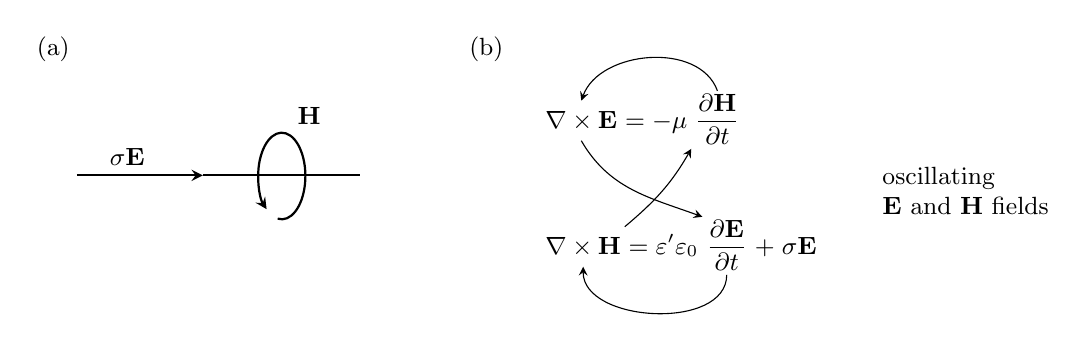
\begin{tikzpicture}[>=stealth, thick, font=\small]
		% (a) current and circulating H
		\begin{scope}
			\node at (-0.3,1.6) {(a)};
			\draw[->] (0,0) -- (1.6,0) node[pos=0.4,above] {$\sigma\mathbf{E}$};
			\draw (1.6,0) -- (3.6,0);
			\draw[->] (2.55,-0.55) arc (-100:230:0.3 and 0.55);
			\node at (2.95,0.75) {$\mathbf{H}$};
		\end{scope}
		% (b) coupled Faraday and Ampere laws
		\begin{scope}[xshift=5.5cm]
			\node at (-0.3,1.6) {(b)};
			% Faraday's law (top row) and Ampere's law (bottom row), built from pieces so arrows can attach
			\node[anchor=base west, inner xsep=1pt] (cE) at (0.4,0.6) {$\nabla\times\mathbf{E}$};
			\node[anchor=base west, inner xsep=1pt] (eqF) at (cE.base east) {$=-\mu$};
			\node[anchor=base west, inner sep=1pt] (dH) at (eqF.base east) {$\dfrac{\partial\mathbf{H}}{\partial t}$};
			\node[anchor=base west, inner xsep=1pt] (cH) at (0.4,-1.0) {$\nabla\times\mathbf{H}$};
			\node[anchor=base west, inner xsep=1pt] (eqA) at (cH.base east) {$=\varepsilon'\varepsilon_0$};
			\node[anchor=base west, inner sep=1pt] (dE) at (eqA.base east) {$\dfrac{\partial\mathbf{E}}{\partial t}$};
			\node[anchor=base west, inner xsep=1pt] at (dE.base east) {$+\;\sigma\mathbf{E}$};
			% Four arrows as in the handwritten sketch, forming a loop:
			% dH/dt drives curl E (Faraday); the curling E is time-varying, dE/dt (feeds Ampere);
			% dE/dt drives curl H (Ampere); the curling H is time-varying, dH/dt (feeds Faraday).
			\draw[->, thin] (dH.north) to[out=110,in=70] (cE.north);
			\draw[->, thin] (cE.south) to[out=-60,in=160] (dE.north west);
			\draw[->, thin] (cH.north east) to[out=40,in=-120] (dH.south west);
			\draw[->, thin] (dE.south) to[out=-90,in=-90] (cH.south);
			\node[anchor=west, align=left] at (4.6,-0.2) {oscillating\\$\mathbf{E}$ and $\mathbf{H}$ fields};
		\end{scope}
	\end{tikzpicture}
	\caption{(a) With $\partial\mathbf{E}/\partial t = 0$, the current $\sigma\mathbf{E}$ produces a magnetic field $\mathbf{H}$ that circulates around it. (b) When $\partial\mathbf{E}/\partial t \ne 0$, Faraday's law and Amp\`ere's law feed each other, producing oscillating $\mathbf{E}$ and $\mathbf{H}$ fields.}
	\label{f:ampere}
\end{figure}

%%%%%%%%%%%%%%%%%%%%%%%%%%%%%%%%%%%%%
\section{EM wave propagation in free space}

\subsection{The wave equation}

In free space, $\sigma = 0$, $\mu = \mu_0$, $\varepsilon' = 1$, and $q_v = 0$, so Faraday's and Amp\`ere's laws become
\begin{equation}
	\nabla\times\mathbf{E} = -\mu_0\frac{\partial\mathbf{H}}{\partial t},
	\qquad
	\nabla\times\mathbf{H} = \varepsilon_0\frac{\partial\mathbf{E}}{\partial t}.
\end{equation}
For the $\mathbf{E}$ field, take the curl of both sides of Faraday's law:
\begin{equation}
	\nabla\times\nabla\times\mathbf{E} = -\mu_0\nabla\times\left(\frac{\partial\mathbf{H}}{\partial t}\right).
\end{equation}
Apply the identity
\begin{equation}
	\nabla\times\nabla\times\mathbf{E} = \nabla(\nabla\cdot\mathbf{E}) - \nabla^2\mathbf{E},
	\qquad (\nabla^2 = \nabla\cdot\nabla \equiv \text{Laplacian}).
\end{equation}
Recalling that Gauss's law (here) is $\nabla\cdot\mathbf{E} = 0$,
\begin{equation}
	\nabla^2\mathbf{E} = \mu_0\frac{\partial}{\partial t}(\nabla\times\mathbf{H}).
\end{equation}
Plugging in Amp\`ere's law gives the EM wave equation in free space:
\begin{equation}
	\label{e:wave_free}
	\nabla^2\mathbf{E} = \mu_0\varepsilon_0\frac{\partial^2\mathbf{E}}{\partial t^2}.
\end{equation}
What does this tell us? The wave speed is
\begin{equation}
	c = \frac{1}{\sqrt{\mu_0\varepsilon_0}} \quad \rightarrow \quad \text{the speed of light}.
\end{equation}
Because $\mu_0$ and $\varepsilon_0$ are universal constants, $c$ is constant for all EM waves in free space.

For the $\mathbf{H}$ field, we can take the same approach to show
\begin{equation}
	\nabla^2\mathbf{H} = \mu_0\varepsilon_0\frac{\partial^2\mathbf{H}}{\partial t^2}.
\end{equation}

\subsection{Uniform plane waves}

Now let's connect these ideas.
\begin{itemize}
	\item Consider a uniform plane wave propagating along $+\hat{\mathbf{z}}$.
	\item For convenience, let us define the electric field in terms of a \emph{phasor} (phase vector) that depends on the spatial coordinates $x$, $y$, $z$:
	\begin{equation}
		\label{e:phasor}
		\mathbf{E}(x,y,z,t) = \mathrm{Re}\left[\tilde{\mathbf{E}}(x,y,z)\,e^{j\omega t}\right],
	\end{equation}
	where $\tilde{\mathbf{E}}$ is the (complex-valued) phasor, $\mathrm{Re}[\cdot]$ denotes the real component of a complex value, and similarly $\mathbf{H}(x,y,z,t) = \mathrm{Re}[\tilde{\mathbf{H}}(x,y,z)\,e^{j\omega t}]$ (recall that $\omega$ is the angular frequency).
	% Phasor box added at the instructor's request (not in the handwritten notes).
	\begin{center}
	\fbox{\begin{minipage}{0.93\linewidth}
		\textbf{Phasors in brief.}
		\begin{itemize}
			\item A quantity oscillating at angular frequency $\omega$, $A(t) = |\tilde{A}|\cos(\omega t + \phi)$, can be written $A(t) = \mathrm{Re}[\tilde{A}\,e^{j\omega t}]$. The \emph{phasor} $\tilde{A} = |\tilde{A}|e^{j\phi}$ packs the amplitude and phase into one complex number.
			\item \emph{Why use them:} $\partial/\partial t \rightarrow j\omega$, which turns time derivatives into algebra.
			\item \emph{Getting back the physical quantity:} multiply by $e^{j\omega t}$ and take the real part. A phasor is not itself the physical field.
			\item \emph{Products need care:} the time average of a product of two such quantities is $\langle A(t)B(t)\rangle = \frac{1}{2}\mathrm{Re}[\tilde{A}\tilde{B}^*]$. This is the origin of the $\frac{1}{2}$ in the time-averaged Poynting vector, Eq.~\eqref{e:poynting}.
			\item \emph{Conventions differ:} we use $e^{j\omega t}$. Some texts, common in physics, use $e^{-i\omega t}$, which flips the sign of imaginary parts (e.g., $\varepsilon = \varepsilon' + i\varepsilon''$).
		\end{itemize}
	\end{minipage}}
	\end{center}
	\item Thus, we have
	\begin{equation}
		\tilde{\mathbf{E}} = \tilde{E}_x\hat{\mathbf{x}} + \tilde{E}_y\hat{\mathbf{y}} + \tilde{E}_z\hat{\mathbf{z}}.
	\end{equation}
	% NOTE: the sentence on separating the vector equation into components was added at the instructor's request
	% (2026-10-08).
	\item Substituting the phasor form into the wave equation, Eq.~\eqref{e:wave_free}, with $\partial/\partial t \rightarrow j\omega$, gives $\nabla^2\tilde{\mathbf{E}} + k_0^2\tilde{\mathbf{E}} = 0$. Because the Cartesian unit vectors $\hat{\mathbf{x}}$, $\hat{\mathbf{y}}$, $\hat{\mathbf{z}}$ do not vary in space, $\nabla^2\tilde{\mathbf{E}} = (\nabla^2\tilde{E}_x)\hat{\mathbf{x}} + (\nabla^2\tilde{E}_y)\hat{\mathbf{y}} + (\nabla^2\tilde{E}_z)\hat{\mathbf{z}}$, so this vector equation separates into three identical scalar equations, one for each component. For $\tilde{E}_x$,
	\begin{equation}
		\left(\frac{\partial^2}{\partial x^2} + \frac{\partial^2}{\partial y^2} + \frac{\partial^2}{\partial z^2} + k_0^2\right)\tilde{E}_x = 0,
	\end{equation}
	% NOTE: handwritten writes the wavenumber as capital K_0 (and K below); written as lowercase k_0, k to match
	% Ulaby & Long (2014, Eqs. 2.16, 4.9) and to avoid K (thermal conductivity) and K (kelvin) in the master table.
	where
	\begin{equation}
		k_0 = \frac{\omega}{c} = \frac{2\pi}{\lambda_0}
	\end{equation}
	is the angular wavenumber in free space and $\lambda_0$ is the wavelength in free space.
	% NOTE: handwritten states only E_y = 0; added E_z = 0 (a uniform plane wave has no field component along its
	% direction of propagation; Ulaby & Long 2014, p. 38), which the following equations assume.
	\item A uniform plane wave has no field component along its direction of propagation ($\tilde{E}_z = 0$), and we hereafter define our coordinate system such that $\tilde{E}_y = 0$.
	\item Because we are considering a uniform plane wave propagating along $\hat{\mathbf{z}}$, we have $\partial^2 \tilde{E}_x/\partial x^2 = \partial^2 \tilde{E}_x/\partial y^2 = 0$, so the wave equation gives
	\begin{equation}
		\label{e:helm_z}
		\frac{\partial^2 \tilde{E}_x}{\partial z^2} + k_0^2 \tilde{E}_x = 0,
	\end{equation}
	% NOTE: handwritten calls this "the general solution"; the general solution also contains a -z-going term
	% E_x^- e^{+j k_0 z} (Ulaby & Long 2014, Eq. 2.22). Reworded to the +z-propagating solution.
	for which the solution for a wave propagating along $+\hat{\mathbf{z}}$ is
	\begin{equation}
		\tilde{E}_x(z) = E_x^+\,e^{-jk_0z}
		\qquad \text{or} \qquad
		\tilde{\mathbf{E}}(z) = E_x^+\,e^{-jk_0z}\,\hat{\mathbf{x}}.
	\end{equation}
	% NOTE: the explanation of the superscript + was added at the instructor's request (2026-10-08); the two-term general
	% solution is U&L 2014, Eq. 2.22.
	The superscript $+$ labels the wave traveling in the $+\hat{\mathbf{z}}$ direction, and $E_x^+$ is its (constant, complex) amplitude at $z = 0$. Eq.~\eqref{e:helm_z} is second order, so its general solution has two terms, $\tilde{E}_x(z) = E_x^+e^{-jk_0z} + E_x^-e^{+jk_0z}$. To see which way each travels, write $E_x^+ = |E_x^+|e^{j\phi^+}$ and return to the time domain: $E_x(z,t) = \mathrm{Re}[E_x^+e^{-jk_0z}e^{j\omega t}] = |E_x^+|\cos(\omega t - k_0z + \phi^+)$. A point of constant phase, $\omega t - k_0z = \text{const}$, moves toward $+z$ as $t$ increases, at speed $\omega/k_0 = c$. Likewise, the $E_x^-$ term moves toward $-z$. Here we consider only the wave traveling along $+\hat{\mathbf{z}}$; we will need both terms when we study reflection at interfaces (Lecture 4).
	\item We can then solve for the corresponding magnetic field by plugging into Faraday's law:
	\begin{equation}
		\tilde{\mathbf{H}}(z) = \frac{1}{\eta_0}E_x^+\,e^{-jk_0z}\,\hat{\mathbf{y}},
	\end{equation}
	where
	\begin{equation}
		\eta_0 = \sqrt{\frac{\mu_0}{\varepsilon_0}} \approx 377\ \Omega
	\end{equation}
	is the \emph{intrinsic impedance} of free space.
	\item For the purposes of comparison, let's rewrite these expressions for $\tilde{\mathbf{E}}$ and $\tilde{\mathbf{H}}$:
	\begin{equation}
		\label{e:plane_free}
		\boxed{
		\tilde{\mathbf{E}}(z) = E_x^+\,e^{-jk_0z}\,\hat{\mathbf{x}},
		\qquad
		\tilde{\mathbf{H}}(z) = \frac{1}{\eta_0}E_x^+\,e^{-jk_0z}\,\hat{\mathbf{y}}
		}
	\end{equation}
\end{itemize}

\subsection{Properties of plane waves}

What do Eqs.~\eqref{e:plane_free} tell us?
\begin{enumerate}
	\item They remind us that $\mathbf{E}$ and $\mathbf{H}$ fields are a package deal: you can't have one without the other (although this was clear from Maxwell's equations).
	% NOTE: handwritten says "H and E are always orthogonal"; qualified to plane waves in isotropic media, which is
	% where Ulaby & Long (2014, Eq. 2.34) state it holds.
	\item They show us that $\mathbf{H} \perp \mathbf{E}$, at least in free space, though this is generalizable to any (isotropic) medium, as we shall see $\Rightarrow$ for plane waves, $\mathbf{H}$ and $\mathbf{E}$ are \underline{always} orthogonal.
	\item $\mathbf{E}$ and $\mathbf{H}$ are in phase, but this is \emph{not} a general property; as we will show, loss (e.g., conductivity) causes a phase shift.
	\item $\mathbf{E}$ and $\mathbf{H}$ are related through the intrinsic impedance.
\end{enumerate}

It can be shown that, in 3D,
\begin{equation}
	\label{e:khat}
	\tilde{\mathbf{E}} = -\eta\,(\hat{\mathbf{k}}\times\tilde{\mathbf{H}}),
	\qquad
	\tilde{\mathbf{H}} = \frac{1}{\eta}(\hat{\mathbf{k}}\times\tilde{\mathbf{E}}),
\end{equation}
where $\hat{\mathbf{k}}$ is the propagation unit vector. This is true for any material with the appropriate definition of $\eta$.

% NOTE: "transverse" qualified to plane waves (Ulaby & Long 2014, p. 39, TEM waves).
The preceding equations make clear that EM (plane) waves are \emph{transverse waves}, meaning they oscillate \emph{only} perpendicular to the direction of propagation (Figure~\ref{f:planewave}). This is a key distinction between EM waves and mechanical waves (e.g., sound waves), which can have longitudinal components.

\begin{figure}[h]
	\centering
	% Illustrative parameters: E_x = cos(k_0 z), eta_0 H_y = cos(k_0 z) (in phase), plotted over two wavelengths.
	% Oblique projection: x-hat up, y-hat toward the lower left, z-hat to the right.
	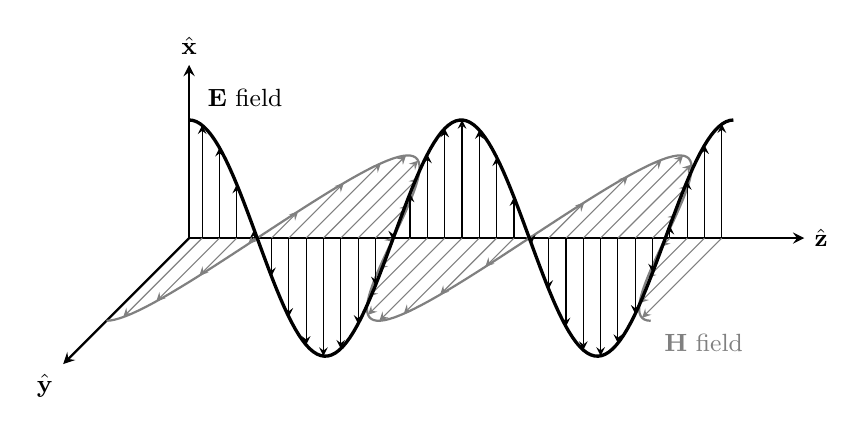
\begin{tikzpicture}[>=stealth, font=\small,
		declare function={ez(\t)=1.5*cos(\t r);}]
		\def\zs{0.55} % horizontal cm per radian of k_0 z
		% axes
		\draw[->, thick] (0,0) -- (0,2.2) node[above] {$\hat{\mathbf{x}}$};
		\draw[->, thick] (0,0) -- (-1.6,-1.6) node[below left] {$\hat{\mathbf{y}}$};
		\draw[->, thick] (0,0) -- (4*pi*\zs+0.9,0) node[right] {$\hat{\mathbf{z}}$};
		% H field (along y): displacement a*(-0.7,-0.7)
		\foreach \t in {0.3,0.7,...,12.5} {
			\draw[->, thin, gray] ({\t*\zs},0) -- ({\t*\zs - 0.7*ez(\t)},{-0.7*ez(\t)});
		}
		\draw[thick, gray] plot[domain=0:4*pi, samples=150] ({\x*\zs - 0.7*ez(\x)},{-0.7*ez(\x)});
		% E field (along x)
		\foreach \t in {0.3,0.7,...,12.5} {
			\draw[->, thin] ({\t*\zs},0) -- ({\t*\zs},{ez(\t)});
		}
		\draw[very thick] plot[domain=0:4*pi, samples=150] ({\x*\zs},{ez(\x)});
		\node[anchor=south west] at ({0.2*\zs},1.55) {$\mathbf{E}$ field};
		\node[anchor=north west, gray] at ({4*pi*\zs - 1.0},-1.1) {$\mathbf{H}$ field};
	\end{tikzpicture}
	\caption{A uniform plane wave in free space propagating along $\hat{\mathbf{z}}$, with $\mathbf{E}$ along $\hat{\mathbf{x}}$ (black) and $\mathbf{H}$ along $\hat{\mathbf{y}}$ (gray), in phase, Eq.~\eqref{e:plane_free}.}
	\label{f:planewave}
\end{figure}

%%%%%%%%%%%%%%%%%%%%%%%%%%%%%%%%%%%%%
\section{EM waves in homogeneous, isotropic, non-ferromagnetic materials}

Now we have $\sigma \ge 0$, $\varepsilon' \ge 1$, $\mu = \mu_0$, and $q_v = 0$.
\begin{itemize}
	\item In free space, we saw that all EM waves travel at the same speed and will travel forever (no attenuation).
	\item What about other materials?
\end{itemize}

\subsection{The wave equation in general media}

Recall Amp\`ere's law, Eq.~\eqref{e:ampere}, and our phasor form for the fields, Eq.~\eqref{e:phasor}. With $e^{j\omega t}$ time dependence, $\partial/\partial t \rightarrow j\omega$, so Amp\`ere's law becomes, in terms of phasors,
\begin{align}
	\nabla\times\tilde{\mathbf{H}} &= j\omega\varepsilon'\varepsilon_0\tilde{\mathbf{E}} + \sigma\tilde{\mathbf{E}} \nonumber\\
	&= j\omega\varepsilon_0\underbrace{\left(\varepsilon' - j\frac{\sigma}{\omega\varepsilon_0}\right)}_{\text{dielectric constant } \varepsilon}\tilde{\mathbf{E}} \nonumber\\
	&= j\omega\varepsilon\varepsilon_0\tilde{\mathbf{E}},
\end{align}
and Faraday's law becomes
\begin{equation}
	\nabla\times\tilde{\mathbf{E}} = -j\omega\mu_0\tilde{\mathbf{H}}.
\end{equation}
Taking the curl of both sides of Faraday's law gives the wave equation in general media,
\begin{equation}
	\label{e:wave_general}
	\boxed{\nabla^2\tilde{\mathbf{E}} - \gamma^2\tilde{\mathbf{E}} = 0,
	\qquad
	\gamma = j\omega\sqrt{\mu_0\varepsilon\varepsilon_0}}
\end{equation}
where $\gamma$ is the complex-valued \emph{propagation constant}. We can derive a similar expression for the $\tilde{\mathbf{H}}$ field, $\nabla^2\tilde{\mathbf{H}} - \gamma^2\tilde{\mathbf{H}} = 0$.

\subsection{Lossless and low-loss media ($\varepsilon \approx \varepsilon'$)}

\begin{itemize}
	\item Define the wavenumber as
	\begin{equation}
		k \equiv \frac{2\pi}{\lambda} = -j\gamma = \omega\sqrt{\mu_0\varepsilon'\varepsilon_0} = \frac{\omega}{c}\sqrt{\varepsilon'} = k_0\sqrt{\varepsilon'}.
	\end{equation}
	\item Thus, the phase velocity of the EM wave is now
	\begin{equation}
		u_p = \frac{\omega}{k} = \frac{c}{\sqrt{\varepsilon'}}.
	\end{equation}
	It is also common to use $n' = \sqrt{\varepsilon'} = c/u_p$, where $n$ is the index of refraction (Section~\ref{s:index}).
	\item The phase velocity shows a couple of important points:
	\begin{enumerate}
		% NOTE: handwritten reads "when eps' = eps(omega)"; corrected to eps'(omega) (missing prime).
		\item $u_p = u_p(\omega)$ when $\varepsilon' = \varepsilon'(\omega)$ $\Rightarrow$ it is common for EM waves to be \emph{dispersive} (waves of different frequencies propagate at different speeds).
		\item $u_p < c$ for $\varepsilon' > 1$.
	\end{enumerate}
	\item Now, following similar steps as before gives the wave equation as
	% NOTE: handwritten reads "dE_x/dz^2"; corrected to the second derivative d^2E_x/dz^2.
	\begin{equation}
		\frac{\partial^2 \tilde{E}_x}{\partial z^2} + k^2\tilde{E}_x = 0,
	\end{equation}
	and the solution takes the form
	% NOTE: handwritten has "E_x" as the amplitude in H(z); corrected to E_x^+ to match E(z).
	\begin{equation}
		\label{e:plane_lossless}
		\tilde{\mathbf{E}}(z) = E_x^+\,e^{-jkz}\,\hat{\mathbf{x}},
		\qquad
		\tilde{\mathbf{H}}(z) = \frac{1}{\eta}E_x^+\,e^{-jkz}\,\hat{\mathbf{y}},
	\end{equation}
	where
	\begin{equation}
		\eta = \frac{\omega\mu_0}{k} = \sqrt{\frac{\mu_0}{\varepsilon'\varepsilon_0}} = \frac{\eta_0}{\sqrt{\varepsilon'}}.
	\end{equation}
	\item[$\bigstar$] Because $\eta$ is real, $\mathbf{E}$ and $\mathbf{H}$ are in phase.
\end{itemize}

\subsection{Lossy media}

Let's add conduction to the mix!
\begin{itemize}
	% NOTE: handwritten reads "Recall wave eq. del^2 E + gamma^2 E = 0 and del^2 H + gamma^2 H = 0"; corrected the sign
	% to -gamma^2 to match Eq. (e:wave_general) and Ulaby & Long (2014, Eqs. 2.13, 2.14).
	\item Recall the wave equations
	\begin{equation}
		\nabla^2\tilde{\mathbf{E}} - \gamma^2\tilde{\mathbf{E}} = 0
		\qquad \text{and} \qquad
		\nabla^2\tilde{\mathbf{H}} - \gamma^2\tilde{\mathbf{H}} = 0,
	\end{equation}
	where
	\begin{equation}
		\gamma^2 = -\omega^2\mu_0\varepsilon\varepsilon_0 = -k_0^2\varepsilon.
	\end{equation}
	\item For convenience (and convention), let's define
	% NOTE: handwritten reads "gamma = alpha + i beta"; corrected to j (course convention j^2 = -1; Ulaby & Long Eq. 4.8).
	\begin{equation}
		\gamma = \alpha + j\beta,
	\end{equation}
	where $\alpha$ is the \emph{attenuation constant} and $\beta$ is the \emph{phase constant}.
	\item For a uniform plane wave propagating along $\hat{\mathbf{z}}$ with the $\mathbf{E}$ field oriented along $\hat{\mathbf{x}}$,
	\begin{align}
		\label{e:plane_lossy}
		\tilde{\mathbf{E}}(z) &= \hat{\mathbf{x}}E_x^+\,e^{-\gamma z} = \hat{\mathbf{x}}E_x^+\,e^{-\alpha z}e^{-j\beta z}, \\
		\tilde{\mathbf{H}}(z) &= \hat{\mathbf{y}}\frac{E_x^+}{\eta}\,e^{-\alpha z}e^{-j\beta z},
	\end{align}
	where
	\begin{equation}
		\label{e:eta_lossy}
		\eta = \frac{\eta_0}{\sqrt{\varepsilon}} = \frac{\eta_0}{\sqrt{\varepsilon'}}\left(1 - j\frac{\varepsilon''}{\varepsilon'}\right)^{-1/2}.
	\end{equation}
	\begin{itemize}
		\item $\beta$ acts as the wavenumber.
		% NOTE: handwritten reads "intensity decays by 1/e over distance delta_s = 1/alpha"; corrected to the field
		% amplitude. Power (intensity) goes as e^{-2 alpha z} and decays by 1/e over delta_p = 1/(2 alpha)
		% (Ulaby & Long 2014, Eqs. 2.63--2.64, 4.10--4.12).
		\item $\alpha$ attenuates: the field amplitude decays by $1/e$ over a distance $\delta_s = 1/\alpha$, where $\delta_s$ is the \emph{skin depth}.
		\item The power (intensity) decays by $1/e$ over the \emph{penetration depth} $\delta_p = 1/(2\alpha)$, so $\delta_s = 2\delta_p$.
	\end{itemize}
	\item Eq.~\eqref{e:eta_lossy} shows us that when $\varepsilon'' > 0$ (e.g., $\sigma > 0$), $\eta$ is complex-valued $\Rightarrow$ phase shift between the $\mathbf{E}$ and $\mathbf{H}$ fields.
\end{itemize}

\subsubsection{Attenuation and phase constants}

Expanding $\alpha$ and $\beta$ gives
\begin{align}
	\label{e:alpha}
	\alpha &= -\omega\sqrt{\mu_0\varepsilon_0}\,\mathrm{Im}\left(\sqrt{\varepsilon}\right)
	= k_0\left\{\frac{\varepsilon'}{2}\left[-1 + \sqrt{1 + \left(\frac{\varepsilon''}{\varepsilon'}\right)^2}\,\right]\right\}^{1/2}, \\
	\label{e:beta}
	\beta &= \omega\sqrt{\mu_0\varepsilon_0}\,\mathrm{Re}\left(\sqrt{\varepsilon}\right)
	= k_0\left\{\frac{\varepsilon'}{2}\left[1 + \sqrt{1 + \left(\frac{\varepsilon''}{\varepsilon'}\right)^2}\,\right]\right\}^{1/2}.
\end{align}
Sanity checks (compare with the lossless case from before):
\begin{itemize}
	\item $\alpha = 0$ when $\varepsilon'' = 0$;
	\item $\beta = k_0\sqrt{\varepsilon'} = k$ when $\varepsilon'' = 0$.
\end{itemize}

\subsubsection{Connecting to the index of refraction}
\label{s:index}

The index of refraction is commonly used in optics and many other fields. It is defined as
% NOTE: handwritten reads "n = n' - j n'' = Re(sqrt(eps)) - j Im(sqrt(eps))", which equals the complex conjugate of
% sqrt(eps). Corrected to n = sqrt(eps) with n'' = -Im(sqrt(eps)) (Ulaby & Long 2014, Eqs. 4.3--4.6), which is what
% the results alpha = k_0 n'' and beta = k_0 n' (their Eq. 4.9) require.
\begin{equation}
	n = n' - jn'' = \sqrt{\varepsilon},
	\qquad
	n' = \mathrm{Re}\left(\sqrt{\varepsilon}\right),
	\qquad
	n'' = -\mathrm{Im}\left(\sqrt{\varepsilon}\right),
\end{equation}
so that, from Eqs.~\eqref{e:alpha} and \eqref{e:beta},
\begin{equation}
	\alpha = k_0 n'', \qquad \beta = k_0 n'.
\end{equation}

%%%%%%%%%%%%%%%%%%%%%%%%%%%%%%%%%%%%%
\section{EM power density: the Poynting vector}

The flow of power (i.e., energy flux) carried by an EM wave is given by the \emph{Poynting vector}
\begin{equation}
	\boldsymbol{\mathcal{S}}(t) = \mathbf{E}(t)\times\mathbf{H}(t) \qquad [\text{W/m}^2].
\end{equation}
Averaged over time, for a uniform plane wave propagating along $\hat{\mathbf{z}}$ (Eq.~\eqref{e:plane_lossy}),
% NOTE: handwritten writes the time average as plain S; written S_av to distinguish it from the instantaneous S(t).
% (Ulaby & Long 2014, Eq. 2.71 use script S with no subscript for the average.)
\begin{equation}
	\label{e:poynting}
	\boldsymbol{\mathcal{S}}_\mathrm{av} = \frac{1}{2}\mathrm{Re}\left[\tilde{\mathbf{E}}\times\tilde{\mathbf{H}}^*\right]
	= \hat{\mathbf{z}}\,\frac{|E_x^+|^2}{2|\eta|}\,e^{-2\alpha z}\cos\phi_\eta,
\end{equation}
where $\phi_\eta$ is the phase of $\eta$ ($\eta = |\eta|e^{j\phi_\eta}$) and $^*$ denotes the complex conjugate. Note the factor of 2 in the exponent for power: power decays twice as fast as the field amplitude.

%%%%%%%%%%%%%%%%%%%%%%%%%%%%%%%%%%%%%
% Symbols follow the master table in ../variables_master.tex; see it for flagged dual usages.
\section*{Variables}

Units are SI. Values are given for universal constants; ``typical'' values are representative, not definitive.

{\small
\renewcommand{\arraystretch}{1.25}
\begin{longtable}{>{$}l<{$} >{\raggedright\arraybackslash}p{0.38\textwidth} >{\raggedright\arraybackslash}p{0.15\textwidth} >{\raggedright\arraybackslash}p{0.24\textwidth}}
\hline
\textrm{Symbol} & Description & Units & Value \\
\hline
\endfirsthead
\hline
\textrm{Symbol} & Description & Units & Value \\
\hline
\endhead
\hline
\endfoot
\multicolumn{4}{l}{\emph{Universal constants}} \\
\varepsilon_0 & permittivity of free space & F/m & $8.854\times10^{-12}$ \\
\mu_0 & permeability of free space & H/m & $4\pi\times10^{-7} \approx 1.257\times10^{-6}$ \\
c & speed of light in a vacuum, $1/\sqrt{\mu_0\varepsilon_0}$ & m/s & $2.998\times10^{8}$ \\
\eta_0 & intrinsic impedance of free space, $\sqrt{\mu_0/\varepsilon_0}$ & $\Omega$ & $\approx 376.7$ ($\approx 120\pi$) \\
j & imaginary unit, $j^2 = -1$ (time dependence $e^{j\omega t}$) & -- & -- \\
\multicolumn{4}{l}{\emph{Constitutive parameters and dielectric properties}} \\
\varepsilon & complex dielectric constant (relative), $\varepsilon' - j\varepsilon''$ & dimensionless & -- \\
\varepsilon' & relative permittivity (real part of $\varepsilon$) & dimensionless & $\ge 1$ (almost always); free space: 1 \\
\varepsilon'' & dielectric loss factor; $\sigma/(\omega\varepsilon_0)$ from conduction & dimensionless & free space: 0 \\
\mu & magnetic permeability & H/m & $\approx\mu_0$ in RS \\
q_v & volume charge density & C/m$^3$ & $0$ in RS \\
\sigma & electrical conductivity & S/m & free space: 0 \\
\omega & angular frequency of the EM wave & rad/s & -- \\
\multicolumn{4}{l}{\emph{Fields and vector calculus}} \\
\mathbf{E} & electric field intensity vector (instantaneous) & V/m & -- \\
\tilde{\mathbf{E}} & phasor of $\mathbf{E}$, $\mathbf{E}(t) = \mathrm{Re}[\tilde{\mathbf{E}}e^{j\omega t}]$ & V/m & -- \\
E_x,\ \tilde{E}_x & $x$-component of $\mathbf{E}$ and of its phasor & V/m & -- \\
E_y,\ \tilde{E}_y & $y$-component of $\mathbf{E}$ and of its phasor & V/m & $0$ (chosen) \\
E_z,\ \tilde{E}_z & $z$-component of $\mathbf{E}$ and of its phasor & V/m & $0$ (plane wave along $\hat{\mathbf{z}}$) \\
E_x^+ & complex amplitude of the $+z$-propagating $\tilde{E}_x$ at $z = 0$ & V/m & -- \\
E_x^- & complex amplitude of the $-z$-propagating $\tilde{E}_x$ at $z = 0$ & V/m & -- \\
\phi^+ & phase of $E_x^+$, $E_x^+ = |E_x^+|e^{j\phi^+}$ & rad & -- \\
\mathbf{H} & magnetic field intensity vector (instantaneous) & A/m & -- \\
\tilde{\mathbf{H}} & phasor of $\mathbf{H}$ & A/m & -- \\
x & Cartesian coordinate & m & -- \\
y & Cartesian coordinate & m & -- \\
z & Cartesian coordinate (direction of propagation) & m & -- \\
\hat{\mathbf{x}} & unit vector along $x$ & dimensionless & -- \\
\hat{\mathbf{y}} & unit vector along $y$ & dimensionless & -- \\
\hat{\mathbf{z}} & unit vector along $z$ & dimensionless & -- \\
t & time & s & -- \\
\nabla & del (gradient) operator & m$^{-1}$ & -- \\
\nabla^2 & Laplacian, $\nabla\cdot\nabla$ & m$^{-2}$ & -- \\
\multicolumn{4}{l}{\emph{Plane-wave propagation}} \\
k_0 & angular wavenumber in free space, $\omega/c = 2\pi/\lambda_0$ & rad/m & -- \\
\lambda_0 & wavelength in free space & m & -- \\
k & angular wavenumber in a lossless or low-loss medium, $k_0\sqrt{\varepsilon'}$ & rad/m & -- \\
\lambda & wavelength in a medium & m & -- \\
\hat{\mathbf{k}} & propagation unit vector & dimensionless & -- \\
\eta & intrinsic impedance of a medium, $\eta_0/\sqrt{\varepsilon}$ & $\Omega$ & real if lossless \\
\phi_\eta & phase angle of $\eta$ & rad & 0 if lossless \\
u_p & phase velocity, $\omega/k$ & m/s & $c/\sqrt{\varepsilon'}$ (low-loss) \\
\gamma & propagation constant, $\alpha + j\beta$ & m$^{-1}$ & $j\omega\sqrt{\mu_0\varepsilon\varepsilon_0}$ \\
\alpha & attenuation constant & Np/m & 0 if lossless \\
\beta & phase constant & rad/m & $k$ if lossless \\
\delta_s & skin depth, $1/\alpha$ & m & $\infty$ if lossless \\
\delta_p & penetration depth, $1/(2\alpha)$ & m & $\delta_s/2$ \\
n & complex index of refraction, $n' - jn'' = \sqrt{\varepsilon}$ & dimensionless & -- \\
n' & real part of $n$, $\mathrm{Re}(\sqrt{\varepsilon})$ & dimensionless & $c/u_p$; free space: 1 \\
n'' & negative imaginary part of $n$, $-\mathrm{Im}(\sqrt{\varepsilon})$ & dimensionless & $\ge 0$ \\
\multicolumn{4}{l}{\emph{Power density}} \\
\boldsymbol{\mathcal{S}} & Poynting vector (instantaneous power density), $\mathbf{E}(t)\times\mathbf{H}(t)$ & W/m$^2$ & -- \\
\boldsymbol{\mathcal{S}}_\mathrm{av} & time-averaged power density, $\frac{1}{2}\mathrm{Re}[\tilde{\mathbf{E}}\times\tilde{\mathbf{H}}^*]$ & W/m$^2$ & -- \\
\end{longtable}
}

\end{document}
